
\documentclass[]{article}
\usepackage{graphicx}
\usepackage{subfigure}
\usepackage{amsmath}
\usepackage{color}
%opening
\title{Report for Computer GraphicII, HW3 \\ Image compression and vectorization by QEM}
\author{Sixun Dong 2021233155 \\ {dongsx@shanghaitech.edu.cn}}


\begin{document}

\maketitle
Acknowledgements:
Deadline: 2022-04-21 23:59:00
\\

You can choose C++ or Python, and no restrictions on programming framework. You can freely use frameworks such as openGL.

The \textbf{report} submits as a PDF file to gradscope, the programming part should package all the files include code, input files, executable file, readme.txt, and report. The \textbf{package} name is  \textbf{your\_student\_name+student\_id.zip}.

You will get Zero if the code not passing the plagiarism check.
\newpage
\section{Image mesh (15 points)}
Implement 2D mesh on the image you selected, describe the data structure of the meshed image.

\paragraph{\color{red}Solution:}
\begin{itemize}
    \item[(1)] Use \textit{matplotlib.patches import Polygon} to generate the triangles.
    \item[(2)] Use list, array and dictionary to save the data of mesh and point.
    \item[(3)] The color of triangle vertices uses it's around pixel colors.
    \item[(4)] The result is as Fig.\ref{fig:q1} shown. 
\end{itemize}
\begin{figure}[ht]
    \centering 
    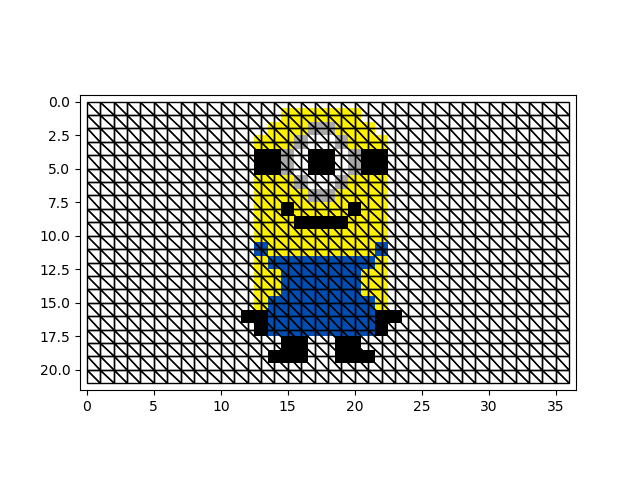
\includegraphics[width=1\columnwidth]{q1.png} 
    \caption{The result of q1.}
    \label{fig:q1} 
\end{figure}

\newpage
\section{Image QEM algorithm (60 points)}
Write down the distance function you chose for the RGB image QEM algorithm, finish your own QEM algorithm and briefly describe the details of your algorithm implementation. Show several results of mesh simplification on different target numbers.
\paragraph{\color{red}Solution:}
I didn't finish all work, I have only done the following.
\begin{itemize}
    \item[(1)] Use the output of Q1 to calculate and first thing is initalization.
    \item[(2)] Use $[x,y,r,g,b]$, 5-dim, to save the information.
    \item[(3)] Traverse all vertices to initalize$A$, $b$, and $c$. Use equation as shown in Fig.\ref{fig:eq1} and \ref{fig:eq2}.
    \item[(4)] Traverse all egdes to initalize the Q. 
    \item[(5)] If it is a non-singular matrix, use the formula in Fig.\ref{fig:eq3}, otherwise use the Fig.\ref{fig:eq4}.
    \item[(6)] If is a singular matrix, need more operations to finish the initalization.
    \item[(7)] Boundary detection done, but not QEM done. There are some bug need to fix, but I didnt finish. All work has submitted in Jupyter nootbook and ZIP.
\end{itemize}
\begin{figure}[ht]
    \centering 
    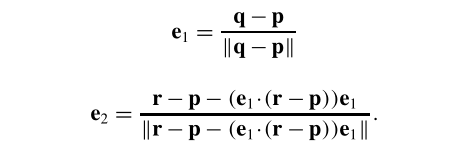
\includegraphics[width=1\columnwidth]{eq1.png} 
    \caption{The equation of $A$, $b$, and $c$.}
    \label{fig:eq1} 
\end{figure}

\begin{figure}[ht]
    \centering 
    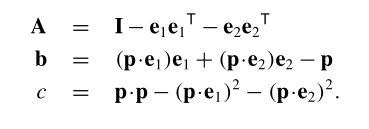
\includegraphics[width=0.8\columnwidth]{eq2.png} 
    \caption{The result of q1.}
    \label{fig:eq2} 
\end{figure}

\begin{figure}[ht]
    \centering 
    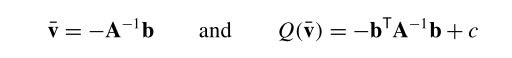
\includegraphics[width=1\columnwidth]{eq3.png} 
    \caption{The result of q1.}
    \label{fig:eq3} 
\end{figure}

\begin{figure}[ht]
    \centering 
    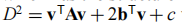
\includegraphics[width=0.5\columnwidth]{eq4.png} 
    \caption{The result of q1.}
    \label{fig:eq4} 
\end{figure}
\newpage
\section{Image zoom in(35 points)}
Select an appropriate QEM target number for the meshed image and implement image zoom in. Compare the result with the original image.

Give up.
\end{document}
